\chapter{Concept and Design}
\label{cha:conceptanddesign}
The goal of this bachelor's thesis is the development of an app for mobile devices, which provides students at TU Berlin the possibility to navigate and inform themselves about their campus in Charlottenburg. The main concept of the mobile app is inspired by popular smartphone navigation systems such as Google or Apple Maps and focuses on mapping TU Berlin's main campus and the most important web resources connected to it onto a single digital map.

\section{Key features and technologies}
The following sections provide a detailed overview of the app's key features (campus map, navigation system and information layer). They furthermore portray the underlying technologies used to develop the mobile application, to query the needed data for the system as well as to perform routing for navigation purposes.

\subsection{Digital map of campus Charlottenburg} \label{campus_map_1}
The main element of the mobile app consists of a locally implemented map of TU Berlin's central campus in Charlottenburg. It provides the user a manageable overview of TU Berlin's buildings, pathways, green areas as well as its surrounding environment. The following list displays possible map features with a description of their relevance for the mobile app:

\begin{itemize}
    \item All buildings of TU Berlin: To provide the user the ability to easily locate the buildings of TU Berlin, all facilities connected to the university need to be specially highlighted on the map. The buildings of TU Berlin are therefore the most important map feature.
    \item All pathways on campus: Footwalks and cycleways that lie on the campus are important for the navigation system of the mobile app. To prevent the map from being cluttered, a hierarchy must be established between important pathways and smaller routes.
    \item All green areas: Parks, trees and other green areas of TU Berlin and its surroundings need to be specially marked on the map. Combined with the buildings and pathways of TU Berlin, they provide the user reference points for manual localization.
    \item External buildings: Buildings not connected to the TU Berlin do not contribute to the localization and navigation on campus. They furthermore take the focus of TU Berlin's campus and are therefore discarded. %They can be nevertheless used as weak informative reference points. A toned-down and subliminal representation on the map can be used in this case.
    \item External pathways: All footwalks and cycleways that are outside of the campus do not provide any relevant information for the mobile app. They furthermore make the map appear more cluttered and are therefore not present on it.
    \item Main roads: Main roads surrounding TU Berlin's campus (e.g., Straße des 17. Juli) simplify the exploration and search process while interacting with the map. They provide an important source of guidance and must be prominently presented on the map.
    \item Small roads: Small roads also support an organized map concept. Since they are less important than main roads, a more restrained manner of display is appropriate. One possibility to achieve this is the usage of toned-down colors combined with a thinner linewidth.
    \item External POI: The POI surrounding the campus (such as Ernst-Reuter-Platz) are heavily recognizable landmarks and support the user's orientation and localization on the map. They are therefore completely included on the map.
\end{itemize}

All relevant features are retrieved via the Overpass-Turbo API from publicly available OpenStreetMap data. The data is then fed into the geographic information system QGIS, which is used for the creation and export of the campus map as well as manual annotation and correction of the downloaded data. Finally, the exported data is converted into a 3d model of the campus which is displayed in a respective rendering environment inside the app (see \hyperref[sub:campus_user_experience]{"Designing a user-friendly campus map"} for more details on the 3d environment).

\subsection{Navigation across the campus}
The mobile app provides the user the ability to easily navigate across TU Berlin's main campus. The most important technological aspects to successfully achieve this task are routing, localization, geocoding, visual presentation of the current navigation state and calculation of estimated time of arrival (ETA). The following sections describe these building blocks in more detail:

Street network graph: The underlying data structure used for the whole navigation process is a weighted graph. Its vertices represent collected geodata points and the respective weighted edges are the distances between the vertices. To account for the fact that, in some cases, the fastest route between two points leads through other buildings, the entrances of all facilities are included in the graph. Every edge connecting a pair of different entrance nodes of the same building is therefore inserted into the graph.

Geocoding: The app's built-in geocoding system provides the ability to convert human-readable input into geocoordinates. This is especially useful when searching for a specific entity on campus by its name or abbreviation. The opposite process is called reverse geocoding. In this case, a set of geocoordinates is taken as input and the closest known entity is returned by the system. This can be for example used to find the closest node in the underlying navigation graph from the user's position.

Localization: The user has two different options when trying to localize himself or a specific entity on the campus. On the one hand, the geocoding provider of the campus app can be used to convert human-readable input into the respective geocoordinates. On the other hand, the user can localize himself with the help of the built-in GPS module of the mobile device. This can be used to determine the user's current position as a starting point for a navigation task.

\newpage

Visual presentation of the navigation process: Similar to already established digital navigation services, a polyline displaying the suggested route is used to visually present the navigation state. It updates accordingly to the user's location and navigation progress (see \hyperref[sub:campus_user_experience]{"Designing a user-friendly campus map"} for further information). Several other user interface elements presenting the total distance and time for the route as well as the ETA support this procedure.

The following figure and sequence present an overview of how the different components work together in the system to provide the navigation functionality of the app:

\begin{figure}[!ht]
	\centering
	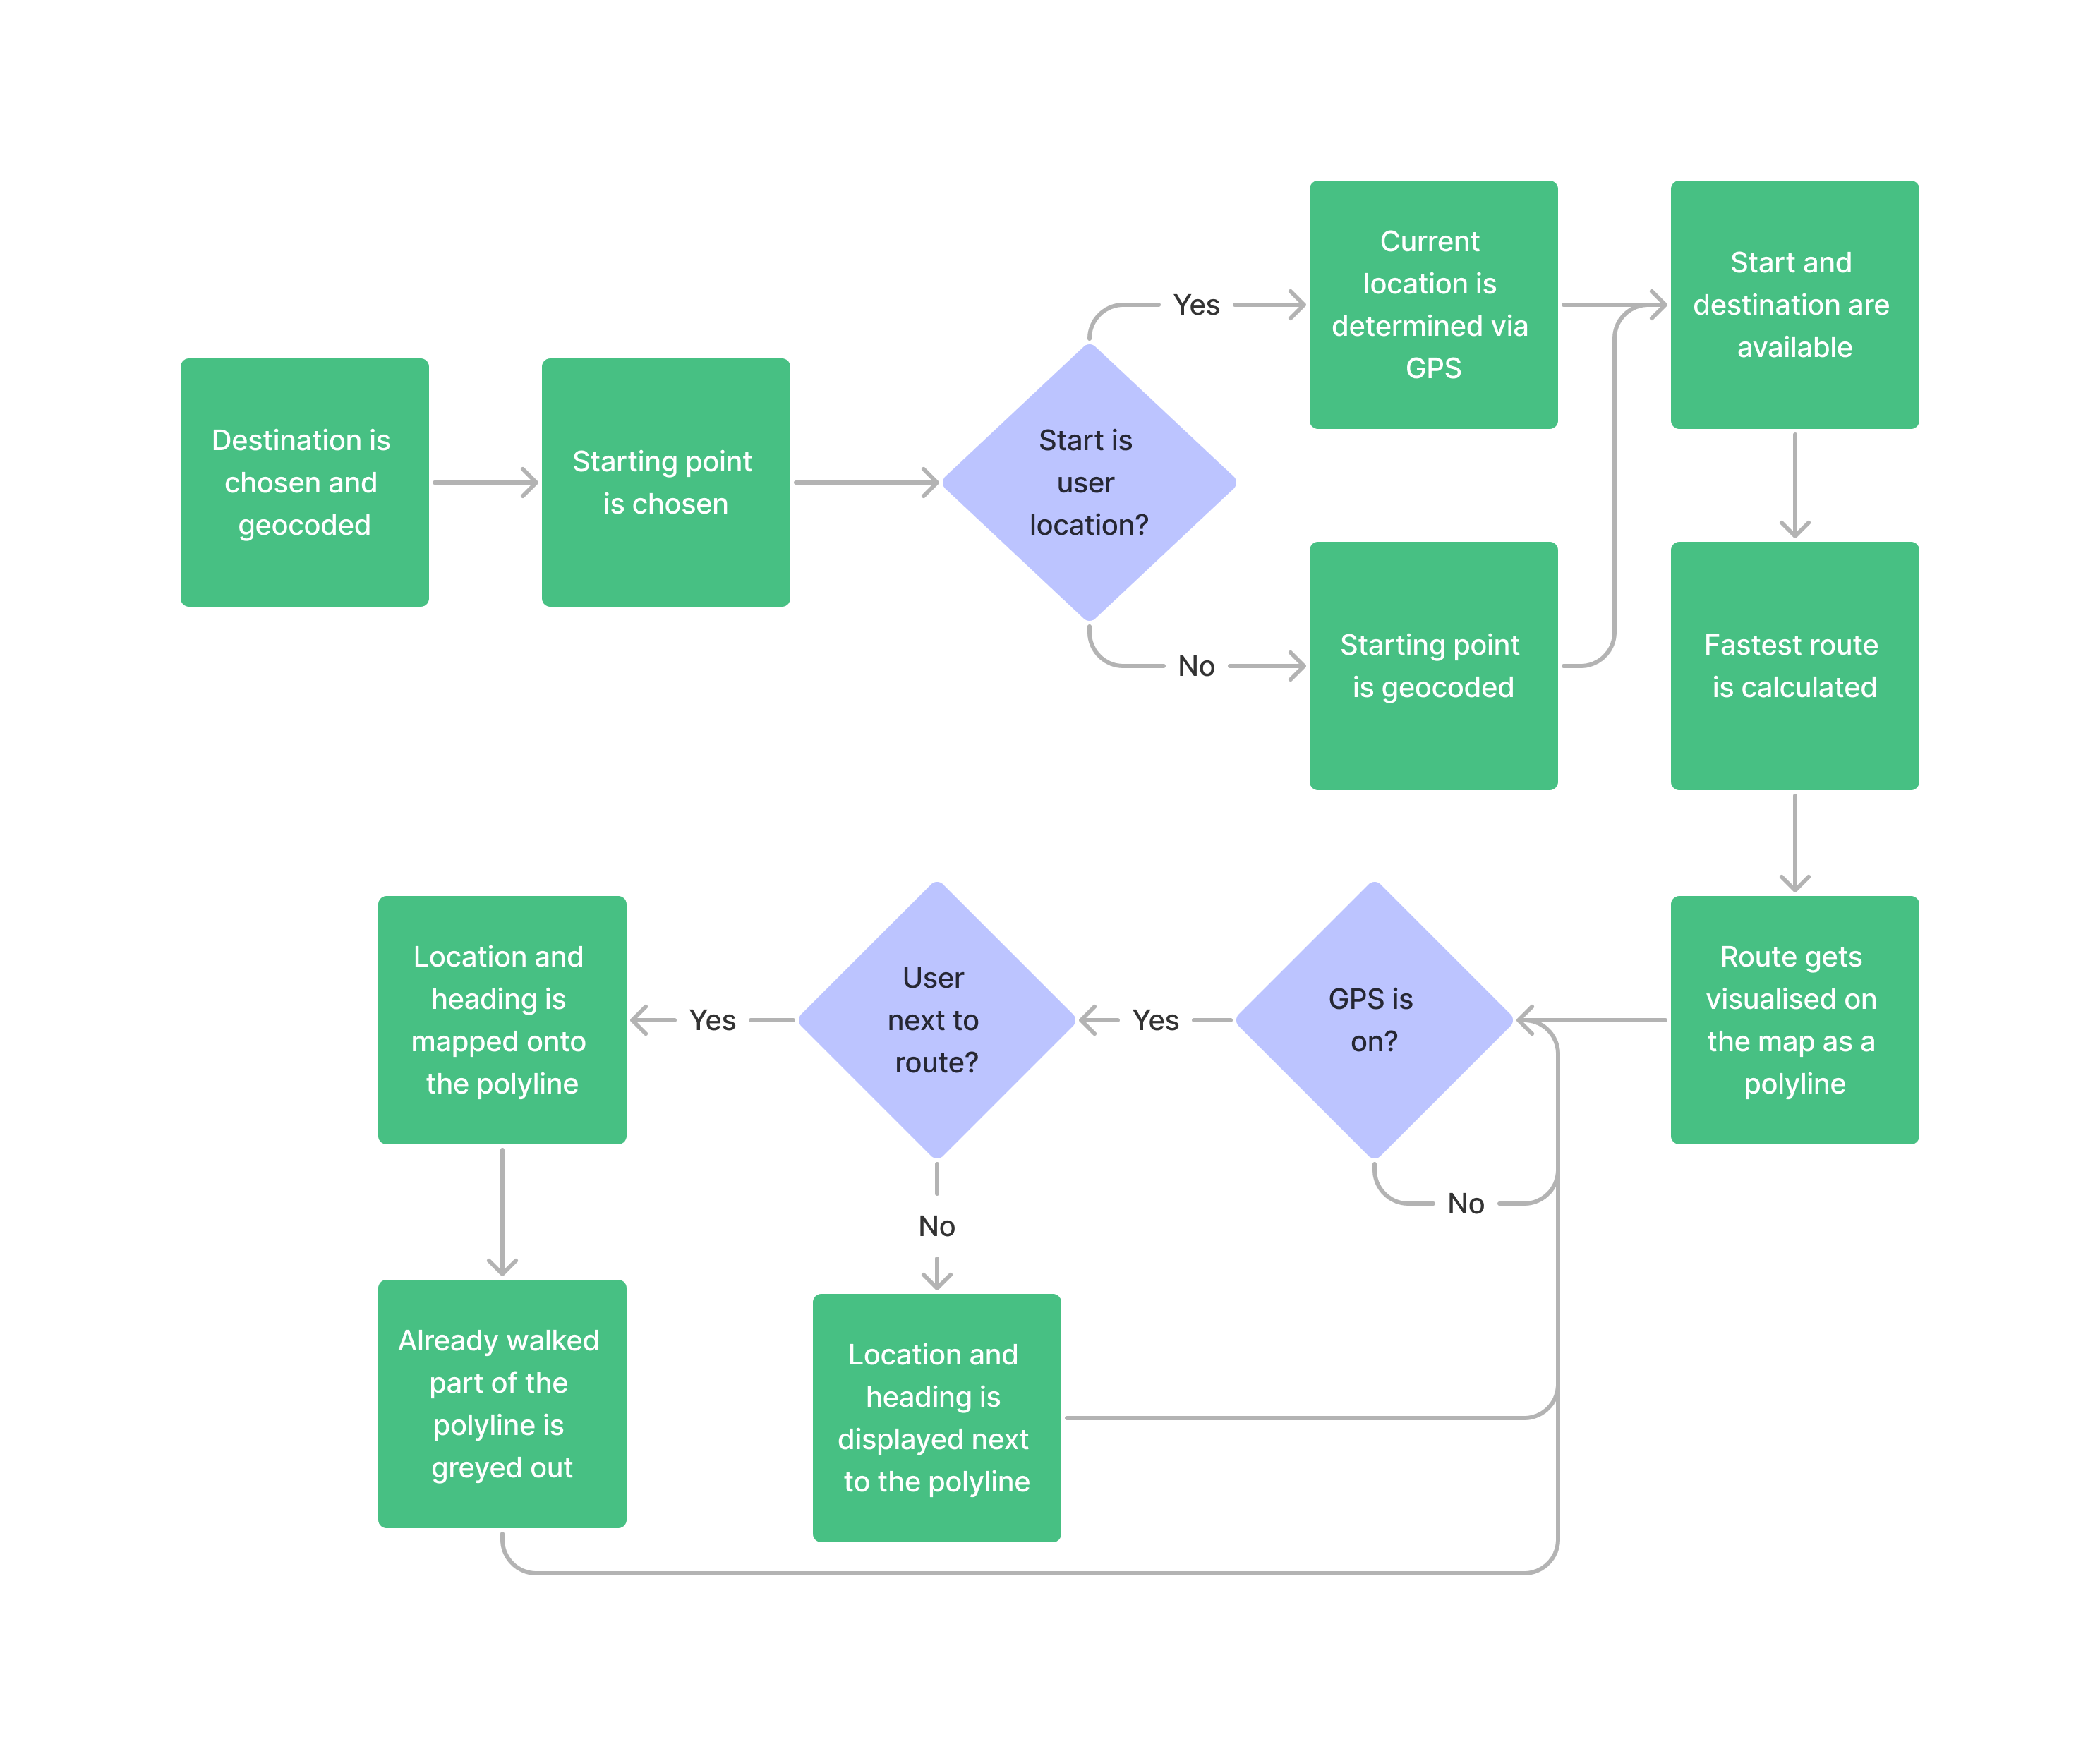
\includegraphics[width=1.0\textwidth]{images/navigation_process.png}\\
	\caption{Complete navigation system procedure}
    \label{fig:navigation_system}
\end{figure}

\begin{enumerate}
    \item Geocoding is used to decode the user's human-readable destination input, e.g., "MAR-Gebäude" into its respective geo-coordinates and node in the graph.
    \item To determine the starting point for the navigation, either another manually inserted location is geocoded or the current location of the user is determined using the built-in GPS module of the mobile phone. If the user selects the latter, the current location and heading are further tracked during the whole navigation process.
    \item Considering the limited size of the graph, Dijkstra's algorithm is chosen to calculate the fastest route between the start and destination points. If the fastest route leads through other buildings, a live indoor navigation approach cannot be achieved due to imprecise GPS results. In this case, geofences are placed on the entrance and exit of the respective building. They detect when the user enters and leaves it and update the state of the navigation system accordingly (see \hyperref[sub:navigation_user_experience]{"Designing a good user experience for navigation"}).
    \item The ETA is calculated based on the weights or distance of the calculated route and other factors (e.g., time of day, stoplights on the route, \ldots).
    \item The navigation is presented visually on the campus map by drawing a polyline of the calculated route. If the user selects its location as a starting point, the current location as well as the heading retrieved from the device's magnetometer is displayed. When the user is located within a certain range of the polyline, its position and heading are mapped onto it.
\end{enumerate}

\subsection{Information layer}
An additional layer on top of the campus map consisting of location-based information is a natural addition to the feature set of the mobile app. It enhances the user experience, the relevance of the whole product and the overall digital information culture of TU Berlin by providing overlays, markers and labels filled with data about the campus.

This section provides a brief overview of the underlying data and technology used to provide the information on the layer.

There are three main sources, that are publicly available and relevant to the information layer. On the one hand, there is the official website of TU Berlin \footnote{https://www.tu.berlin}, with sections for current events, the latest news, deadlines, etc. On the other hand, there is the MOSES system \footnote{https://moseskonto.tu-berlin.de/moses/index.html} containing data about all the different courses, rooms and studies. Lastly, the website of Studierendenwerk Berlin \footnote{https://www.stw.berlin} with meal plans for its different canteens and a timetable for events can be seen as a third important source of information.

Information is collected by downloading and parsing the content of respective websites. The data is further categorized and -if possible- mapped onto different POIs on the campus map (e.g., a canteen gets its meal plan assigned), which provides an intuitive and organized way for information access and display.

The collected data can be categorized according to its timeliness and the intervals in which it has to be updated: General information about different fields of study, courses and rooms only changes by semester. This particular data can be retrieved once at the start of every semester and does not need daily live updates. It is also possible to supply it via app updates, instead of providing a direct in-app functionality for data retrieval. Data that gets updated regularly on the other hand, e.g., meal plans, events, news, etc. has to be always retrievable from the app.

The proposed solution for timely data (meals, events, \ldots) collection and provision runs on a web server and consists of a web crawler for information retrieval, parsing and POI mapping, a database to store the crawled information in a standardized and simple-to-use format and a REST API, that provides the client/mobile device the ability to retrieve the information. One web crawler is used per data category and is triggered periodically by a respective CRON job, whose timing is dependent on the timeliness of the crawled data (see figure \ref{fig:summary_data_retrieval} for summary).

Web crawlers dealing with data that needs rare updates (rooms, buildings, courses, \ldots) on the other hand, are not deployed on a web server. These programs are designed for manual usage at the beginning of a semester and provide their scraped data in JSON format, which can be directly included in the mobile app. This results in the fact that all data falling under this category can be used on the client side without the need for a network connection. It also means that some sort of deployment system needs to be included in the app for this data: Either the information is stored on a web server and gets automatically downloaded and stored on the client's device at the beginning of a semester or a complete app update from the respective app stores is rolled out.

By splitting the logic for crawling and provision, the workload that arises on TU Berlin's and Studierendenwerk's websites from retrieving data can be limited to a minimum: The server only crawls data when an update is needed (e.g., daily for meal plans), instead of loading and parsing the web resources on client request. Further advantages are the fact that loading times for requests from clients are independent of TU Berlin's and Studierendenwerk's infrastructure, that the language for web crawling can be chosen independently from the programming framework (in this case Python with its Selenium \footnote{https://www.selenium.dev} and BeautifulSoup \footnote{https://pypi.org/project/beautifulsoup4} libraries are used) and that the web crawling logic can be changed without updating the app.

\begin{figure}[H]
	\centering
	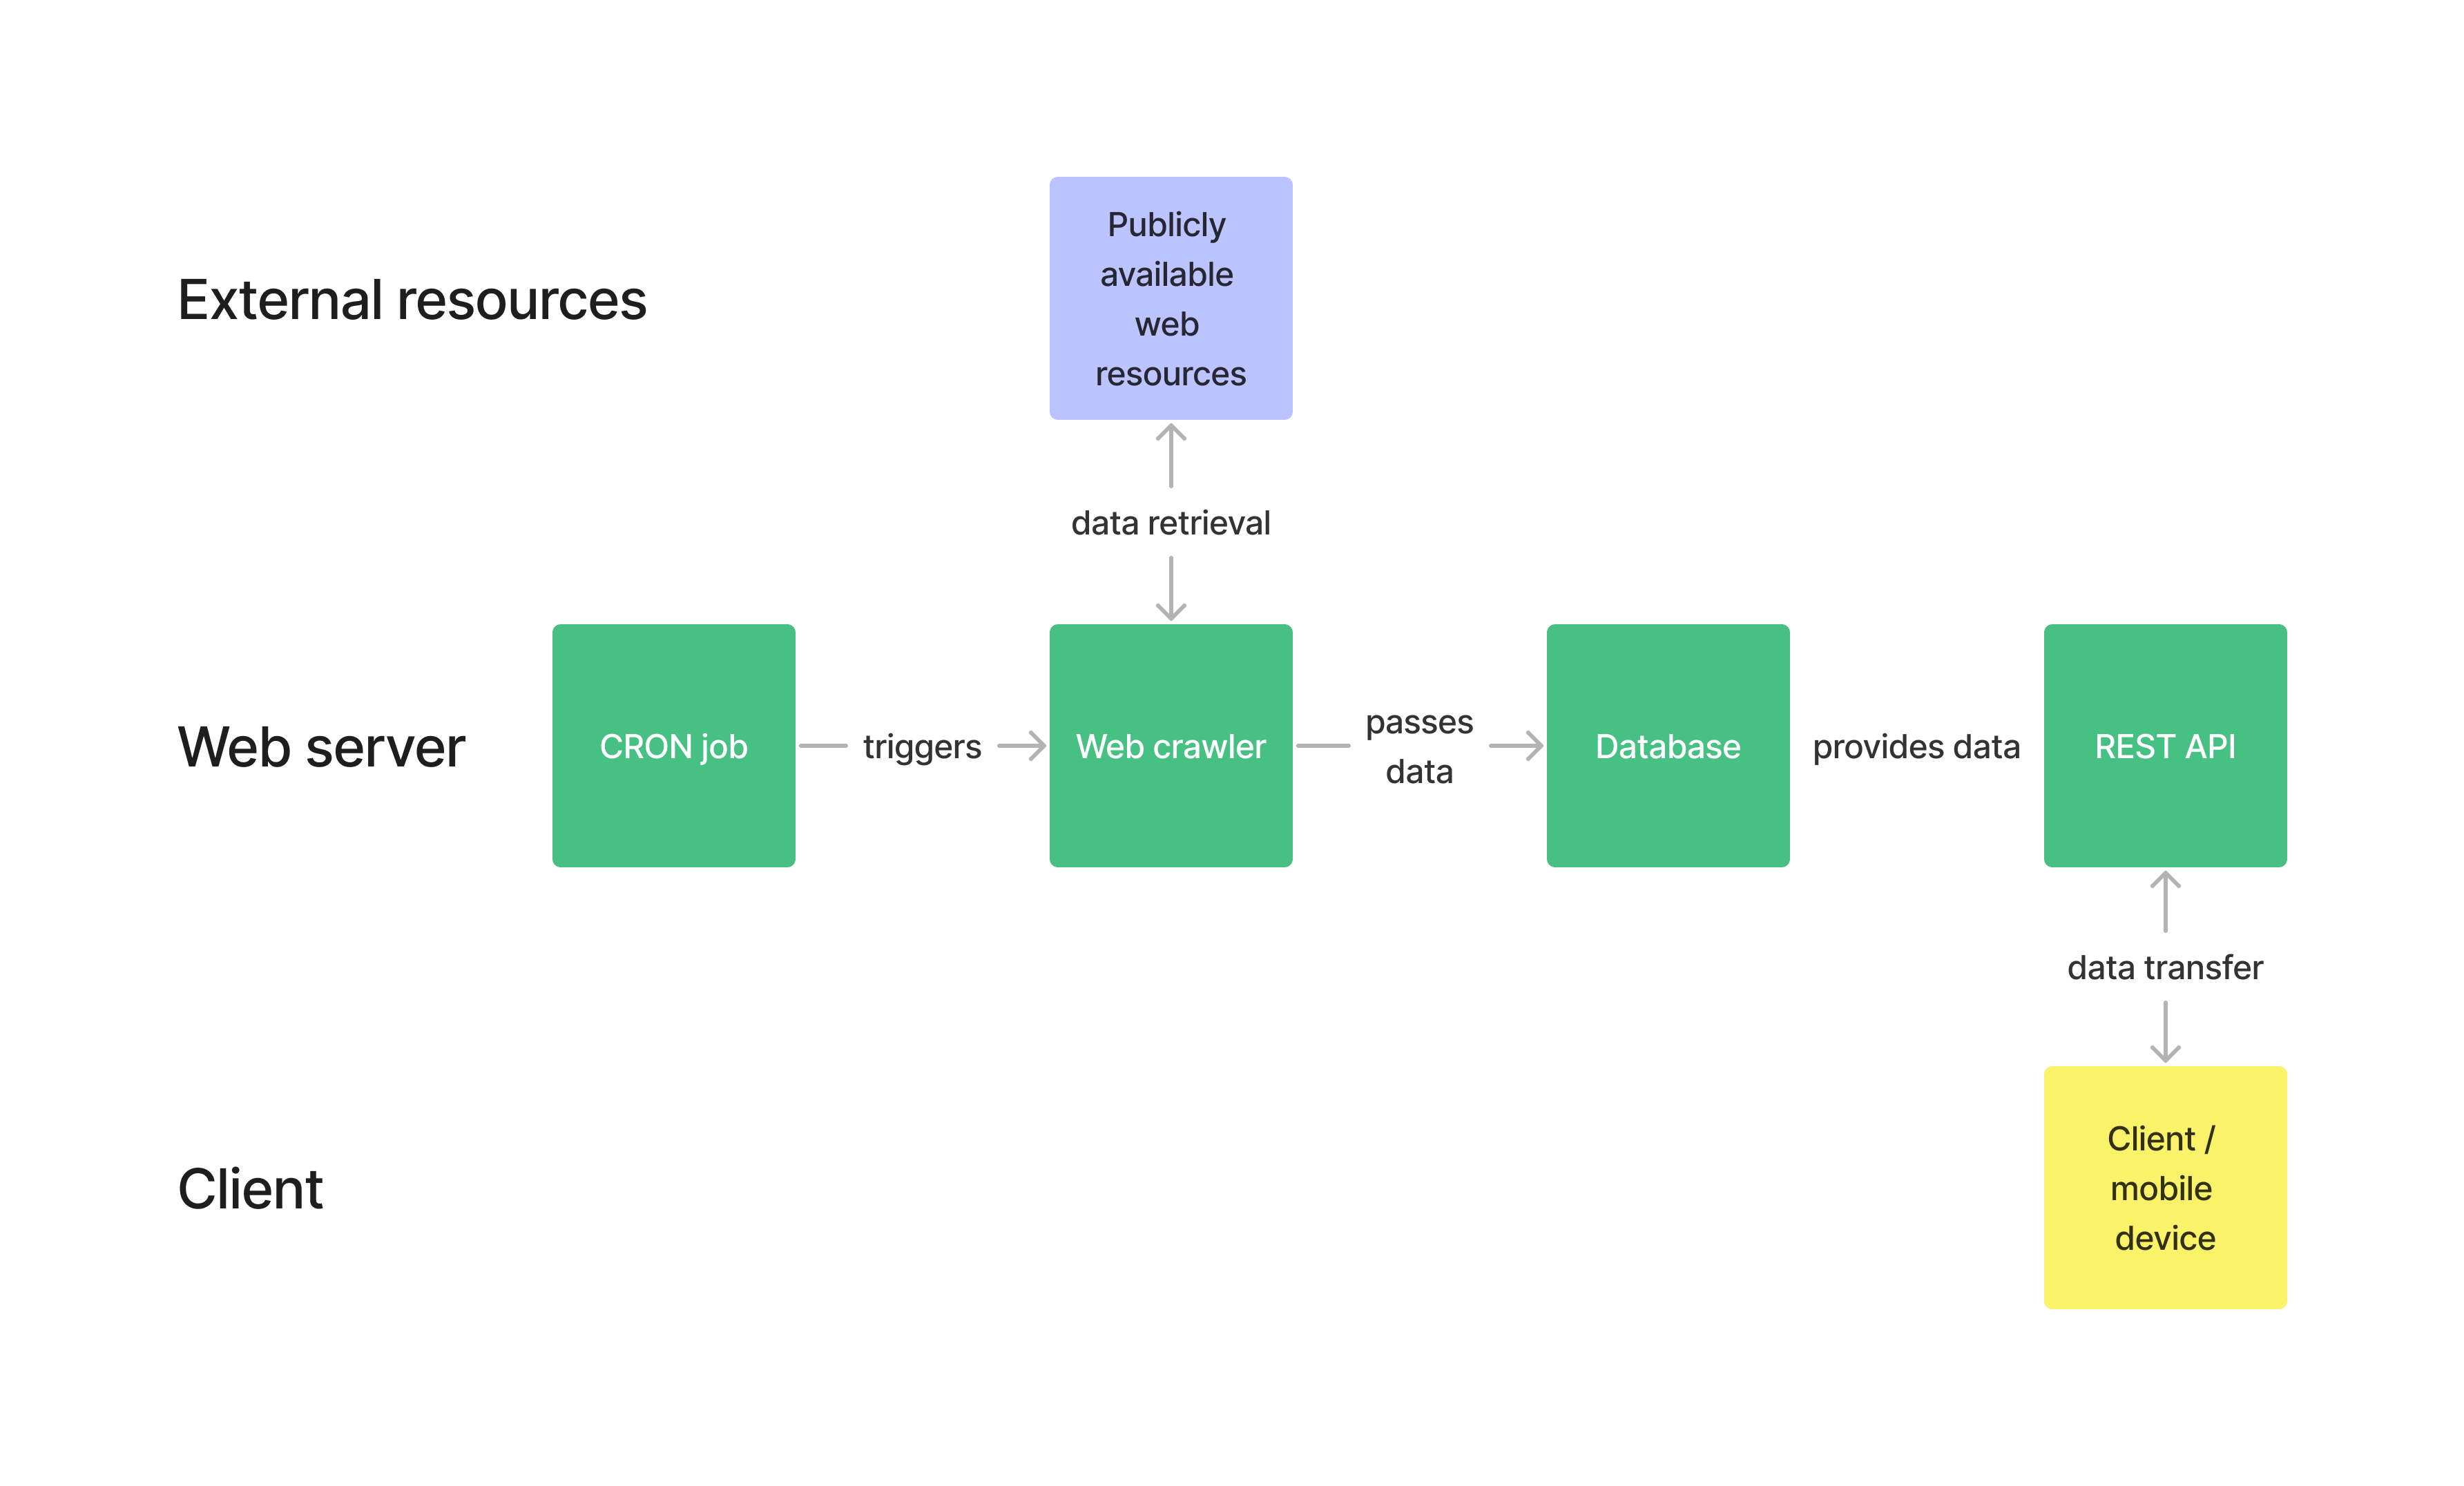
\includegraphics[width=1.0\textwidth]{images/data_retrieval_process.png}\\
	\caption{Data retrieval process for the information layer}
    \label{fig:summary_data_retrieval}
\end{figure}

%\subsection{Exploration vs. search}
%\subsection{Search functionality}
%\subsection{Alternative presentation of information}

\subsection{Offline-first design}
One important aspect of the app concept is an extensive focus on offline usability. The whole system is designed to allow the user (as far as possible) app usage without the need for a network connection. This applies in particular to the navigation system, the campus map and the information layer of the app:

Campus map: The campus map is locally implemented on the device. All necessary information can be therefore loaded and used without a network connection.

Navigation system: Due to the comparatively small scope of the navigation system, the weighted graph for navigation as well as the system for routing can both be implemented and executed on-device. Only the navigation feature working with live user location updates relies on stable GPS functionality.

Information layer: Loading and presenting information on TU Berlin's main campus requires access to the respected online resources and cannot be realized without a network connection. The need for network connectivity can be nevertheless reduced: Since most of the data does not require real-time updates (the most critical data being meal plans that require daily updates), the data for the information layer can be stored locally after download and loaded from memory for the remaining day. This approach reduces the need for internet connectivity to a minimum.

%This can be realized by sending silent push notifications at the start of every week. Devices that cannot receive the synchronizing push notification can download the data while being used. At best, this system allows the user to use the app throughout the week without going online.

\section{App development framework}
The choice of app development framework is an important step while conceptualizing and designing the product. It determines the programming language of the project, the built-in device- and system-specific capabilities that can be accessed during development as well as the performance of the app. It has to be selected in consideration of the project's requirements. The following enumeration presents the most important demands for this thesis:
\begin{itemize}
    \item Used technologies: Working with low-level hardware and operating system APIs is an important part of development. Technologies and systems used in the key features of the product (e.g., GPS capabilities) have to be accessible or implemented in the selected framework.
    \item Cross-platform capabilities: Native app development is complex and time-consuming. Learning and especially working with two different codebases (Java / Kotlin for Android, Swift / Obj. C for IOS) is difficult and not possible within the scope of this thesis. Cross-platform frameworks solve this problem by providing the ability to work with a single codebase for different operating systems.
    \item Focus on high-quality user interfaces: A clear, modern and responsive user interface is a key factor for shipping a high-quality user experience. The availability to easily build such user interfaces is therefore an important requirement for the app development framework. 
    \item Execution speed: Regarding the fact that the whole navigation functionality has to take place locally on the phone, the speed with which the code of the mobile app gets executed is crucial to a responsive and fast user experience. Particularly the algorithms used for routing have to be reliably computable within fractions of a second.
    \item 3d rendering capabilities: The framework needs to provide a way to render and interact with the created 3d model of campus Charlottenburg. Further built-in systems such as an extensive linear algebra toolkit, a lighting engine and other real-time rendering capabilities also need to be taken into account.
\end{itemize}

Based on the previously defined requirements, the Flutter framework \footnote{https://flutter.dev} is chosen for this work. In addition to its cross-platform capabilities, it also offers the ability to compile source code into platform-specific machine code for near-native execution performance. It further comes with access to thousands of packages through the dart package manager pub \footnote{https://pub.dev}, an extensive set of pre-built components for user interfaces and the ability to write platform-specific code for low-level API access. Since Flutter lacks 3d rendering capabilities, the Unity engine \footnote{https://unity.com/de} is additionally used to create and display the campus map. It gets included in the Flutter build and is responsible for rendering and interacting with the 3d campus map.

\section{User experience design}
The following sections provide an overview of the whole user experience (UX) design for the campus app. In the scope of this thesis, the complete process is broken down into UX research and wireframe design.

UX research is a process where the main goals and tasks associated with the app are identified and broken down into its most relevant UX aspects. This helps to find out the key usability requirements for the visual user interface design, consisting of wireframes and high-fidelity mockups (user interface design).

Wireframes, on the other hand, form the first visual version of the app design. They determine the basic structure of the app, its layout, the placement of basic user interface elements as well as their hierarchy. Wireframes are based on the previously defined usability requirements in the UX research process.

It is important to notice that all these design choices are not chosen arbitrarily, but rather based on previous research in the studies of user experience design. Important work was contributed over the years by psychologists and researchers like Dr. Jakob Nielsen \cite{jakob_nielsen}, Dr. Paul Fitts \cite{paul_fitts}, Jon Postel and research conducted at IBM and Xerox Corporation. An overview of the most important research and its consequences for user experience design can be found in Jon Yablonski's book "Laws of UX" \cite{yablonski2020laws} (web-version \cite{yablonski_web}).

The next paragraphs describe a set of important usability requirements that are then further incorporated into the wireframe design.

\subsection{Search versus exploration}
One of the most important usability requirements for the app results from the clash of two important user needs, namely search and exploration. These needs result from the fact that users may use the app for different purposes and with different expectations.\\

Search, on the one hand, describes a scenario, in which the user tries to find or locate a specific piece of information within the app. This search for information can be expressed with concrete questions, e.g.:

\begin{itemize}
    \item What is the fastest way between MAR and TEL buildings?
    \item What are the opening times of the TU library?
    \item What food can I get tomorrow at the main cafeteria?
    \item Where does course App-Entwicklung take place?
    \item In which building is the SNET department located?
\end{itemize}

One main requirement for the user experience of the app is therefore the possibility for fast, easy and structured access to important key information about TU Berlin's campus. Based on \cite{fitts_law} and \cite{jakobs_law}, all search-task-related user interface elements should be easily identifiable as such, prominently positioned and accessible to the user. Additionally, to reduce the search time for the seeking person, the design should also provide multiple ways to access the most important information. Important user interface elements in this case are search bars, descriptive icons and textual hints as well as an adequately chunked information hierarchy in the whole app. This usage of commonly used user interface elements also supports \cite{jakobs_law}.\\

Exploration, on the other hand, is an app use case, in which the user "just browses around" in search of nothing particular. The seeking person either wants to learn, find out or experience something new or uses the app with an open question in mind. In this scenario, the user does not seek a specific piece of information but rather expects the app to provide the possibility, to easily navigate and view through structured content without the need for a concrete search.

Examples of goals and questions for exploration use cases can be the following:

\begin{itemize}
    \item Are there any interesting places on TU Berlin's campus that I could visit?
    \item Which cafeteria has the best food today?
    \item Are there any appealing courses, outside of the scope of my studies, that I can attend this semester?
    \item Search for upcoming events by TU Berlin or Studierendenwerk
    \item Search for learning spaces at TU Berlin
\end{itemize}

In these use cases, the outcome of the exploration action is often determined by the subjective preferences of the users. The app therefore cannot give an optimal final solution to the search but rather present a set of information, from which the user can select or find the most suitable one.

This results in two important requirements for the app design. Firstly, visual elements for the structured presentation of information need to be used. These elements help the user by giving hints about existing information in the app and by structuring related information, which then can be easily overviewed and potentially compared while exploring. Further motivation for this can be found in principles \cite{jakobs_law}, \cite{law_of_common_region}, \cite{hicks_law} and \cite{millers_law}. Examples of such elements can be tables, scrollable lists, clearly designed information cards and different kinds of markers on the campus map.

Secondly, the choice of which information is portrayed in the app is important. Since too much information provision risks a bloating of the app (and therefore leads to a reduced user experience) \cite{hicks_law}, the final campus data needs to be carefully selected and filtered for in-app usage. The establishment of a clear hierarchy between important, frequently used data and less important information also contributes to this.

\subsection{Designing a user-friendly campus map} \label{sub:campus_user_experience}
A precise and clear map of TU Berlin's main campus in Charlottenburg is the most important user interface element in the app. Accordingly, special emphasis should be placed on the design of it. This section describes possible requirements for the map element and the resulting implications for its appearance and implementation in the app.

There are two intended ways how the users should interact with the map: Interaction for exploration/search tasks and interaction for navigation purposes. Both these tasks come with separate design requirements.

Exploration and search tasks, mainly interacting with POI and buildings on TU Berlin's campus, have a strong focus on its entities. A straightforward map design with a focus on the recognizability of buildings, pathways, natural areas and POI is important. This supports the user's need for orientation and simplifies the process of matching real-life buildings with their counterparts on the digital map, which is proven to enhance the user experience \cite{jakobs_law}.

This mostly differs from popular available mobile navigation services since their primary tasks are navigation and orientation of the user. They are also laid out for presenting huge areas, e.g., districts or even complete cities. A detailed portrayal of a specific area is therefore not feasible, perfomant or necessary.

The campus map only deals with a pre-defined and small area. This provides the possibility for the creation of a detailed and complex map, with a pleasing aesthetic (based on \cite{aesthetic_usability_effect}) and a strong focus on TU Berlin's entities on campus Charlottenburg. To achieve maximum recognition value for the buildings, parks and pathways on the campus, a 3D overview, similar to TU Berlin's campus plan \cite{campus_plan}, is used for portrayal. This is especially beneficial for users who are familiar with the official campus plan of TU Berlin, who can transfer their learning from the manual map onto the digital one, which plays well with \cite{jakobs_law}. The 3D perspective also lays out a clear emphasis on buildings, which are the most important entities on the campus and prominently stick out on the map. It is nevertheless also beneficial for other entities, which can be more easily localized with the buildings.

To direct the focus even more onto TU Berlin's campus, all of its surroundings are not used in the 3D view (based on \cite{law_of_common_region}). Furthermore, all important buildings are labeled with their respective abbreviations through markers on the map. Lastly, the user also gets the possibility to alter the map view between 2D and 3D modes, so that the preferred style of view can be selected.

Another important aspect is the zoom range the user can utilize while interacting. Considering that the campus area is small and that the app wants to focus on its details, a close zoom, with a little room maneuver should be appropriate.

Navigation tasks, namely interacting with / following a polyline route and working with a marker that displays the current user location, have a strong focus on pathways and routes on TU Berlin's main campus. It is therefore important to highlight these routes in the design accordingly. Other entities like buildings, natural areas (green areas, water) and POI have a lower priority in this case but are nevertheless important for orientation purposes. To design for this use case one can take inspiration from already established mobile map services like Google Maps \footnote{https://developers.google.com/maps?hl=de} and Apple Maps \footnote{https://www.apple.com/de/maps}. These apps mainly display the road network, important markers and POI while in navigation mode and only present low-priority entities (e.g., outlines of buildings) on a close zoom level.

\begin{figure}[H]
	\centering
	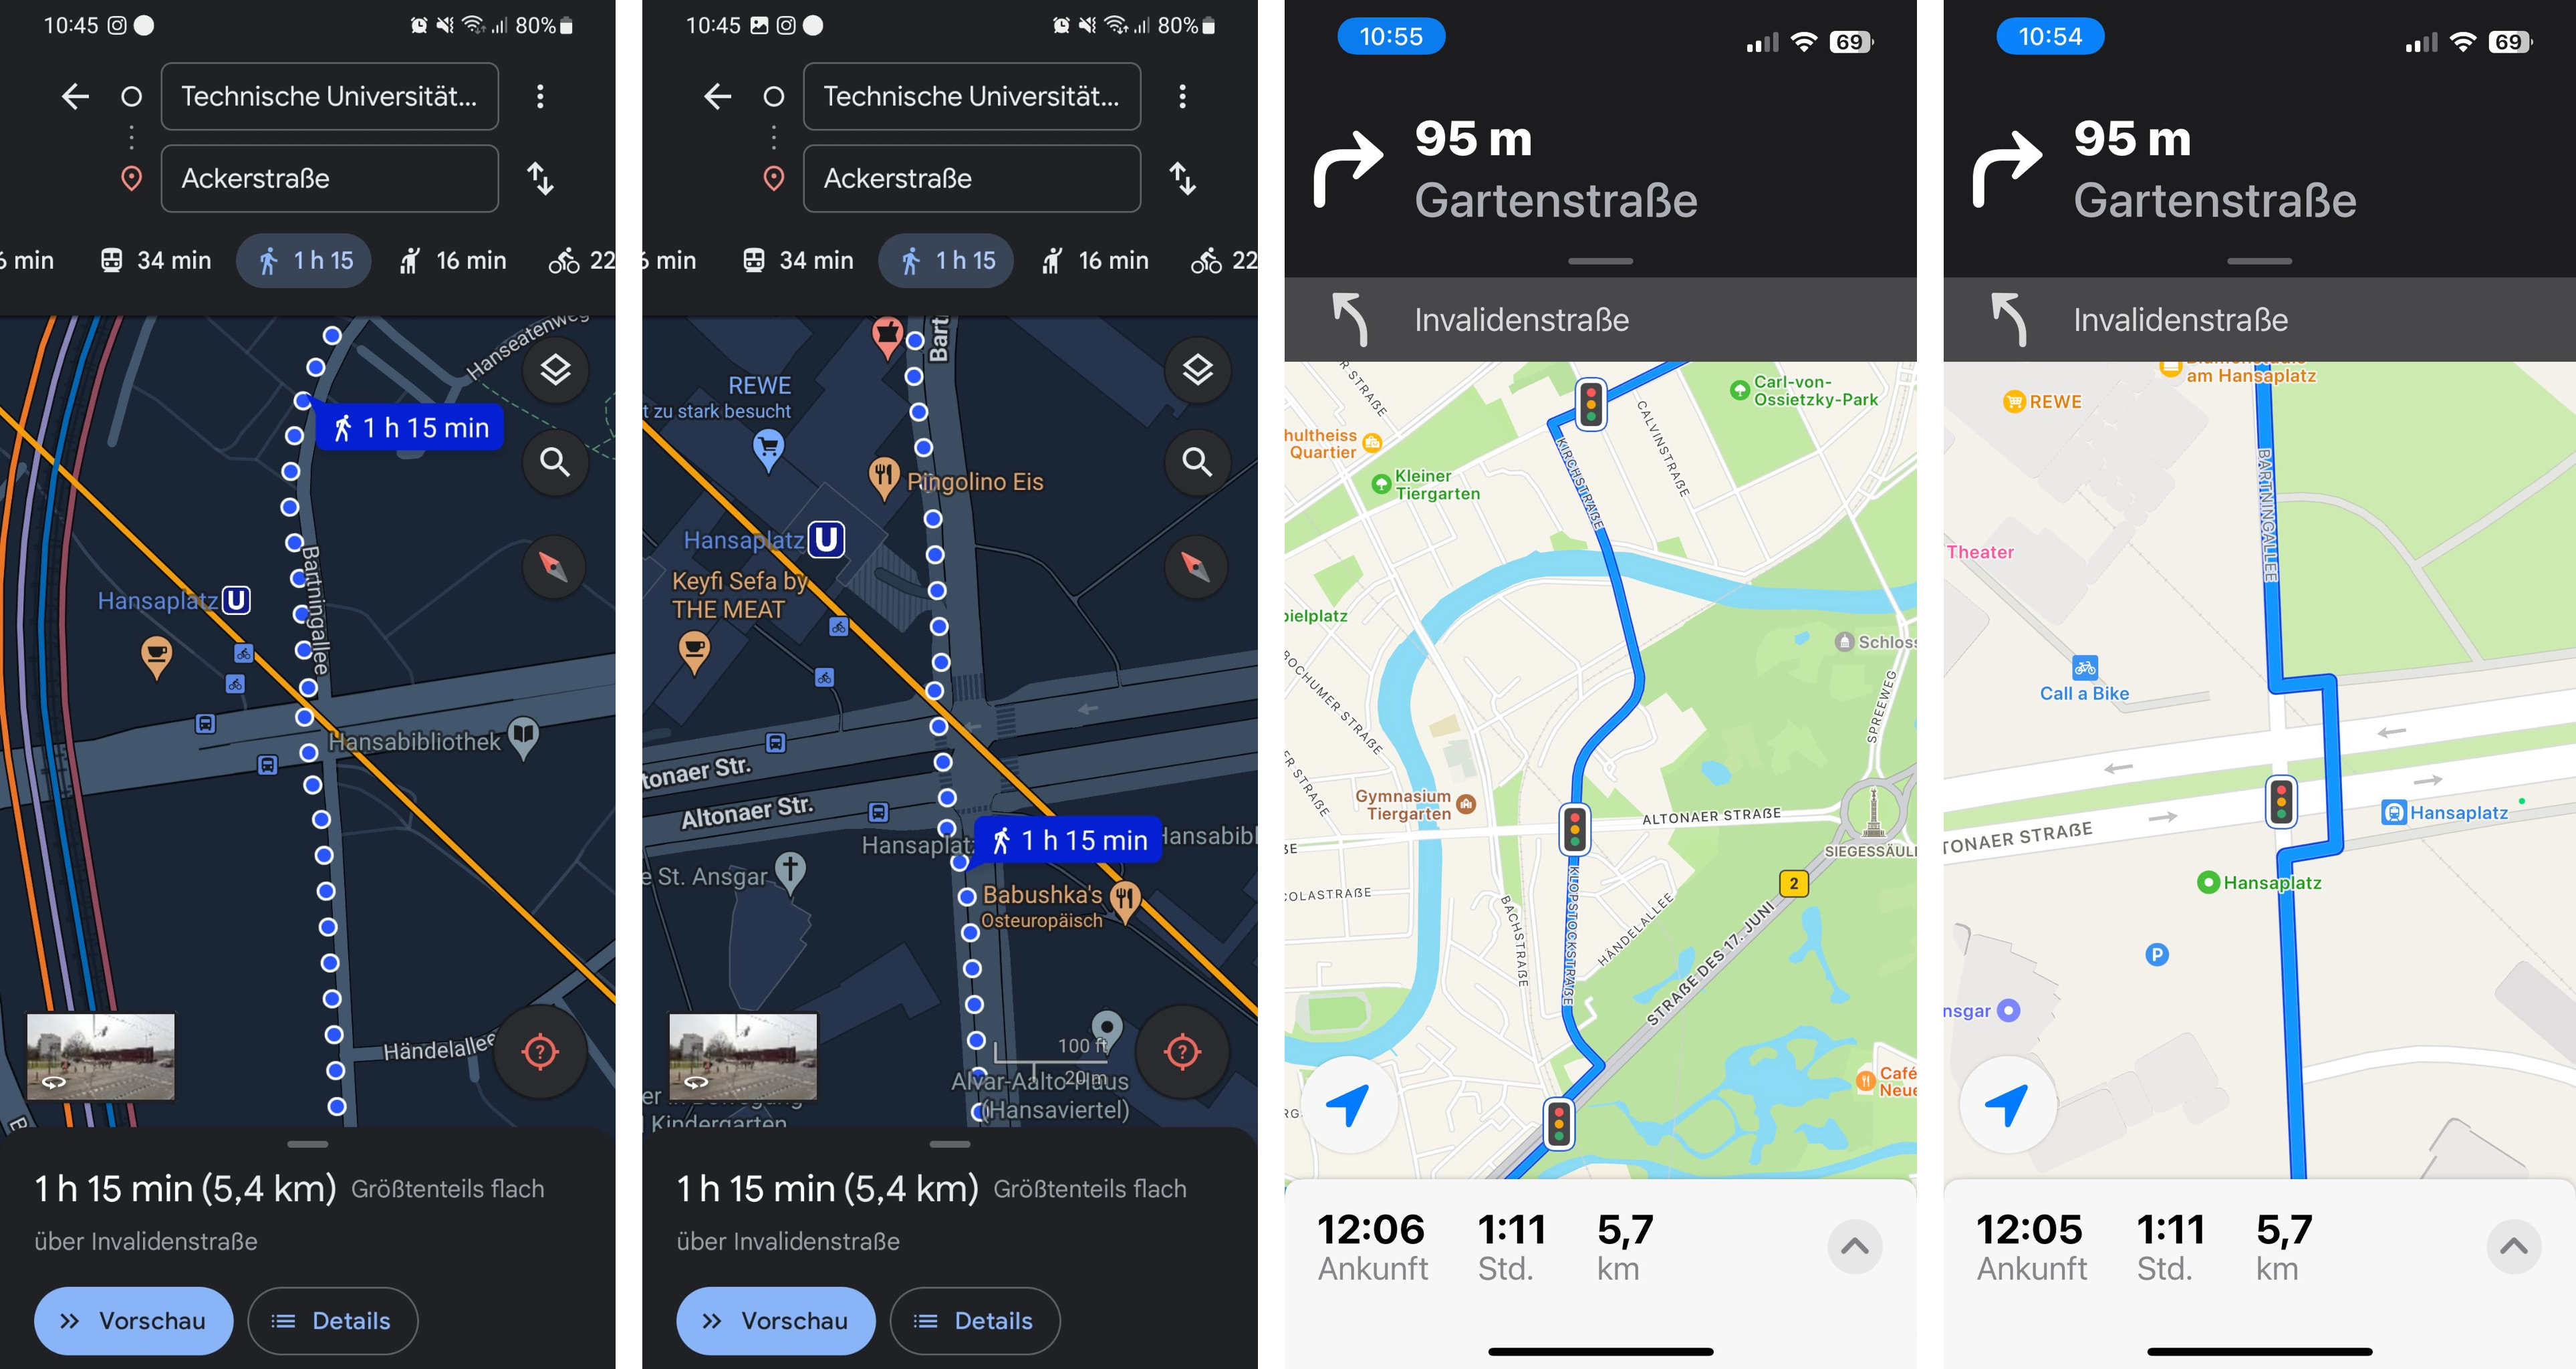
\includegraphics[width=0.85\textwidth]{images/map_design_google_apple.png}\\
	\caption{Different styles of map presentation in Google Maps and Apple Maps}
\end{figure}

Based on the fact, that common usability patterns are already established by the user base of such popular mobile navigation services, the approach is adopted in this thesis (enhancement of user experience based on \cite{jakobs_law}): The user's focus is directed to the road network during the navigation phase, unimportant markers are discarded, roads are highlighted and the map's camera is adjusted to display a 2D perspective from the top.

\subsection{Designing a good user experience for navigation} \label{sub:navigation_user_experience}
Creating a robust and easy-to-use digital navigation system is a challenging task since it consists of digital instructions resulting in real-life actions.

Based on \cite{jakobs_law}, it is beneficial for the user experience to orientate the design to industry standards. In this case, a polyline is usually used for the display of the calculated route, a round marker stands for the user's position and a change in color of the polyline tracks the already traveled path segment. The location marker is further mapped onto the polyline during navigation, as it marks the point between the traveled and preceding route.

Nevertheless, one important difference between established navigation systems and campus navigation is the fact that the latter can also lead through buildings of TU Berlin. Since the app only detects whether (and where) the user enters or leaves a building (the traditional polyline approach is therefore not feasible) and the user base is likely not familiar with a switch from outdoor to indoor navigation, a robust and clear user experience has to be provided during this phase.

To specify the design requirements for this section of the navigation process, the outdoor indoor switch can be broken down into a set of phases, each with its demands:

%The app should be designed in a way that ...

\begin{enumerate}
    \item The user is outdoors during the navigation phase or examines a precalculated route and sees an (upcoming) segment that leads through a building: In this case, the user must understand that a segment leads through a building. It should be furthermore clear which entrance has to be used. The latter can be achieved by marking the entrance position on the map, either with a model of a door (3D perspective) \cite{jakobs_law} or a marker containing an appropriate icon (2D perspective). To clarify the indoor section even more, the polyline of the route should be connected to the entrance and a descriptive marker (e.g., "upcoming indoor section") or other indication should be next to the indoor segment. This repetitive "announcing" of an upcoming indoor section is strongly connected to \cite{teslers_law} and \cite{law_of_proximity} and an enhancement of user experience can be therefore expected. It is important to notice that due to \cite{postels_law}, the user should not be punished in a scenario, where a wrong entrance is taken into the correct building. The app should simply continue the navigation in this case.
    \item The user walks into the marked entrance of the building and is now indoors, the app registers this: In this phase, the biggest explanation part is fulfilled, the user has understood that the next segment is indoors and has entered the building successfully. It is now important to provide the user a visual feedback, that strengthens his correct choice of entering the building ("Great, you have found your way into the building!"), updates the progress on the route accordingly (due to \cite{goal_gradient_effect}) and explains that there is no indoor localization available. The use of animation is a great tool to indicate a change in the state of a user interface. In this case, the map moves and zooms to the entered building and a non-moving marker appears, indicating that the user is inside of the building. A pop-up appears, explaining the location of the user and its goal to find a specific exit of the building.
    \item The user is inside of the building: No specific changes to the user interface need to be made, the app waits till the user has found the exit. In an optimized scenario, an additional pop-up could be triggered if the user spends too long inside the building and searching for the exit. This pop-up would display additional information for finding the desired exit (enhances the UX according to \cite{teslers_law}).
    \item The user walks out of the building and is now outdoors, the app registers this: This phase should reverse the changes made when entering the building. The navigation continues on the polyline with a reappearing location marker, the map unlocks the focus on the exited building, and all markers and pop-ups for indoor navigation disappear. The user gets the feeling that he has successfully made it through the indoor section and can now continue his journey outdoors. Just like in the entering phase and according to \cite{postels_law} the user should also not be punished when taking the wrong exit in the building. In this case, the app should simply detect the wrong exit, recalculate the route from the new user position and display this in the user interface.
\end{enumerate}

%\begin{figure}[H]
%	\centering
%	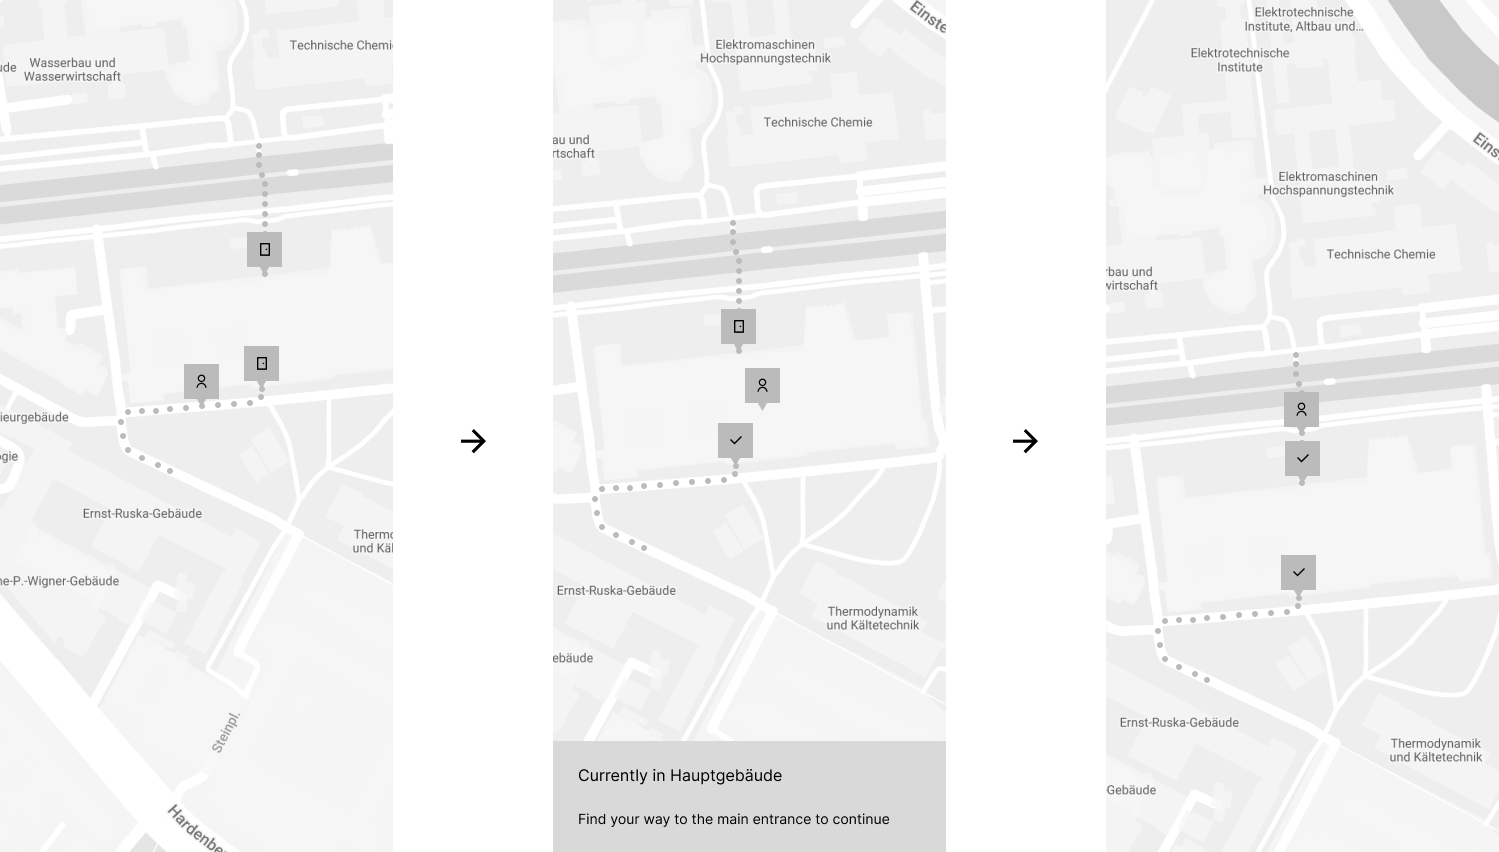
\includegraphics[width=0.35\textwidth]{images/indoor_navigation_phases.png}\\
%	\caption{UX design for outdoor-indoor-outdoor transition}
%\end{figure}

\subsection{Chunking of information within the app}
According to \cite{millers_law}, an organized visual information structure is key to providing a good user experience. Especially concerning the fact that a huge amount of campus data is available and exploration tasks are key activities in the app. Chunking is the task of grouping related information visually together and is a key enabler for an organized layout \cite{millers_law}. The following figure provides a clustered overview of the available data connected to TU Berlin's main campus:

\begin{figure}[H]
	\centering
	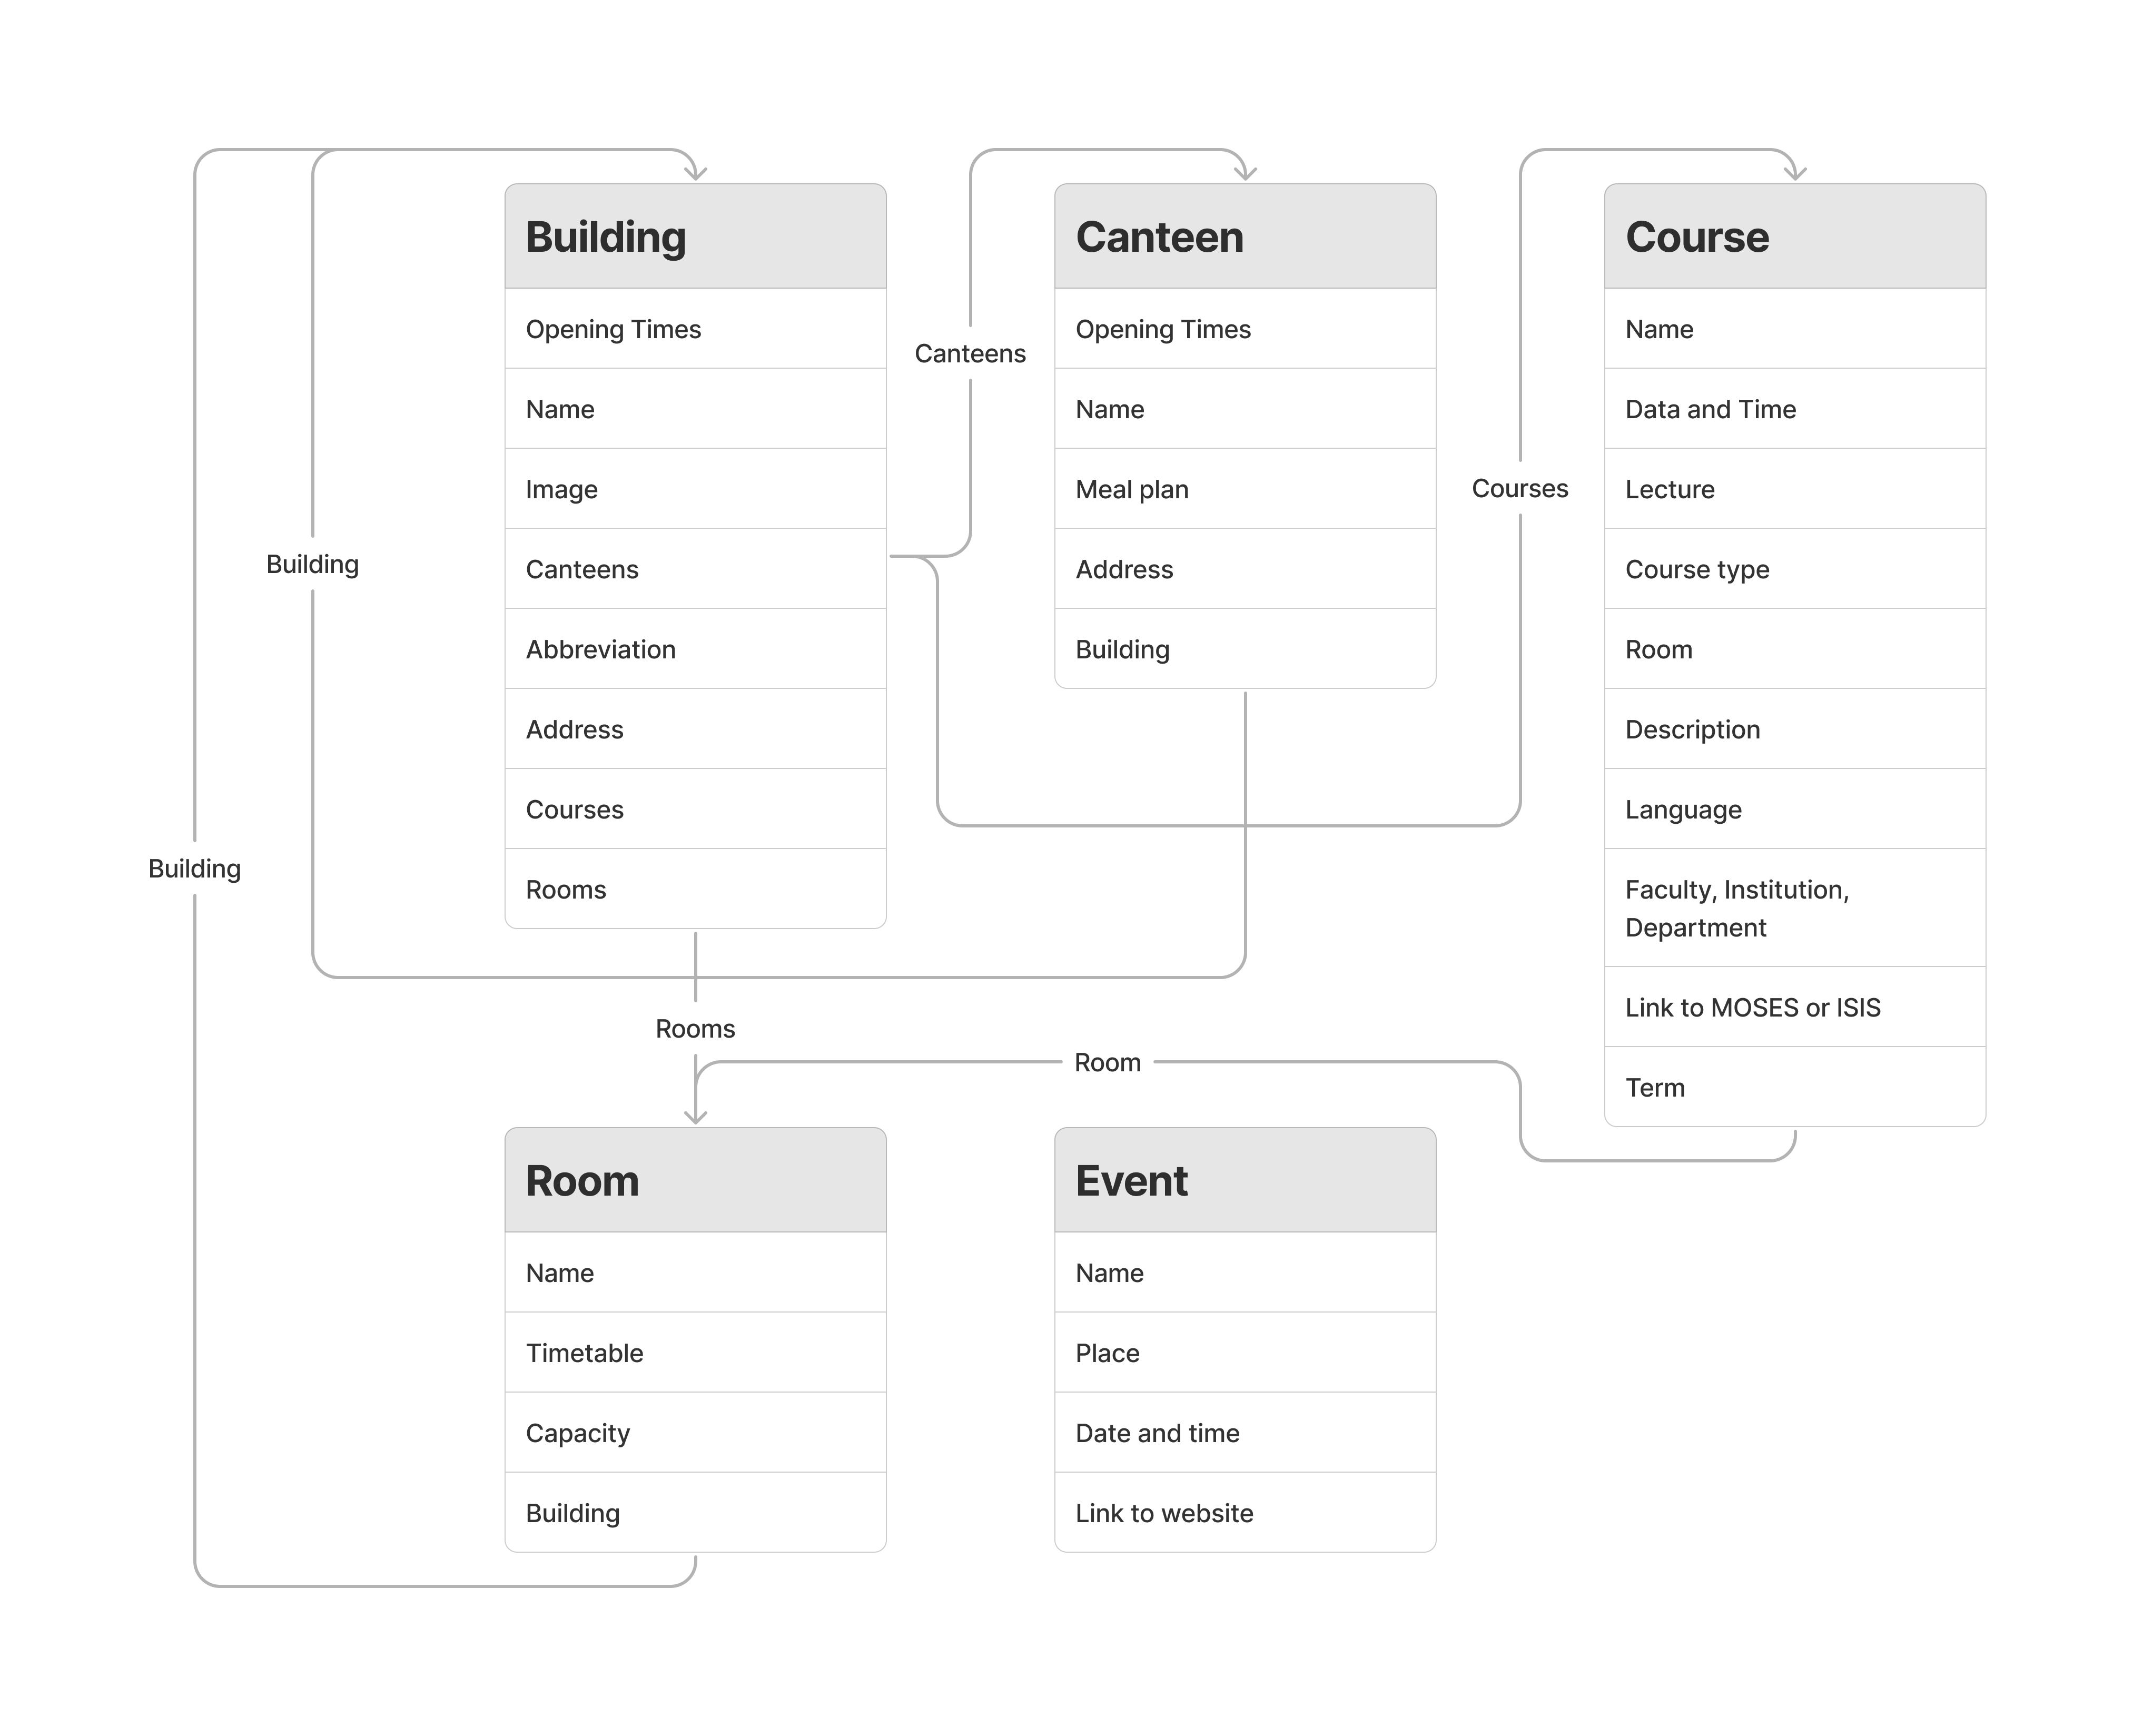
\includegraphics[width=0.85\textwidth]{images/information_cluster.png}\\
	\caption{Clustered data of TU Berlin with their relationships}
\end{figure}

Based on connection count and data, the "Building" and "Course" clusters can be identified as key entities in the system. It is therefore advisable, to attach importance to the display of these groups in the user interface of the app. Other groups are therefore placed less prominently but also get referenced (according to the relations in the figure) in places where "Building" and "Course" are portrayed.

According to \cite{law_of_common_region} and \cite{law_of_similarity}, it is advisable to display information related to one common cluster next to each other and similarly. This improves the user experience by emphasizing associated information. The comprehensibility of the visual design is also important: The user should directly understand the meaning of the portrayed data, which can be mainly achieved with descriptive texts and iconography.

\newpage

\subsection{Wireframes}
Based on the previously defined requirements, wireframes outlining the basic design concept of the app are created. This section displays the most important pages and provides a brief enumerated overview of their features. (Note that not all wireframes are presented and that certain design and layout changes occur between UX and UI design.)

\begin{figure}[H]
	\centering
	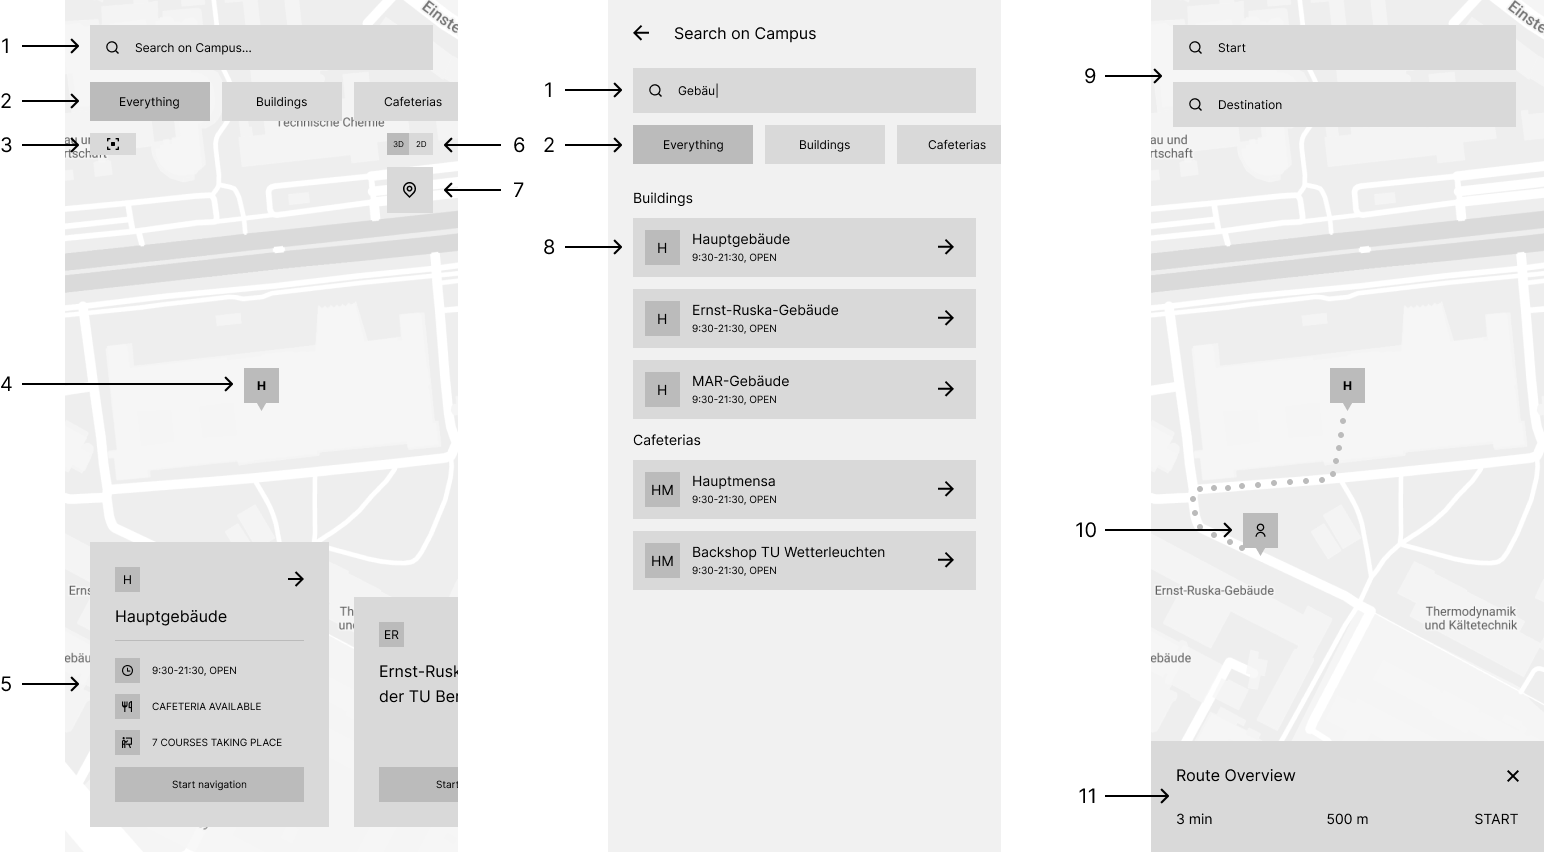
\includegraphics[width=0.9\textwidth]{images/wireframes_1.png}\\
\end{figure}

\begin{figure}[H]
	\centering
	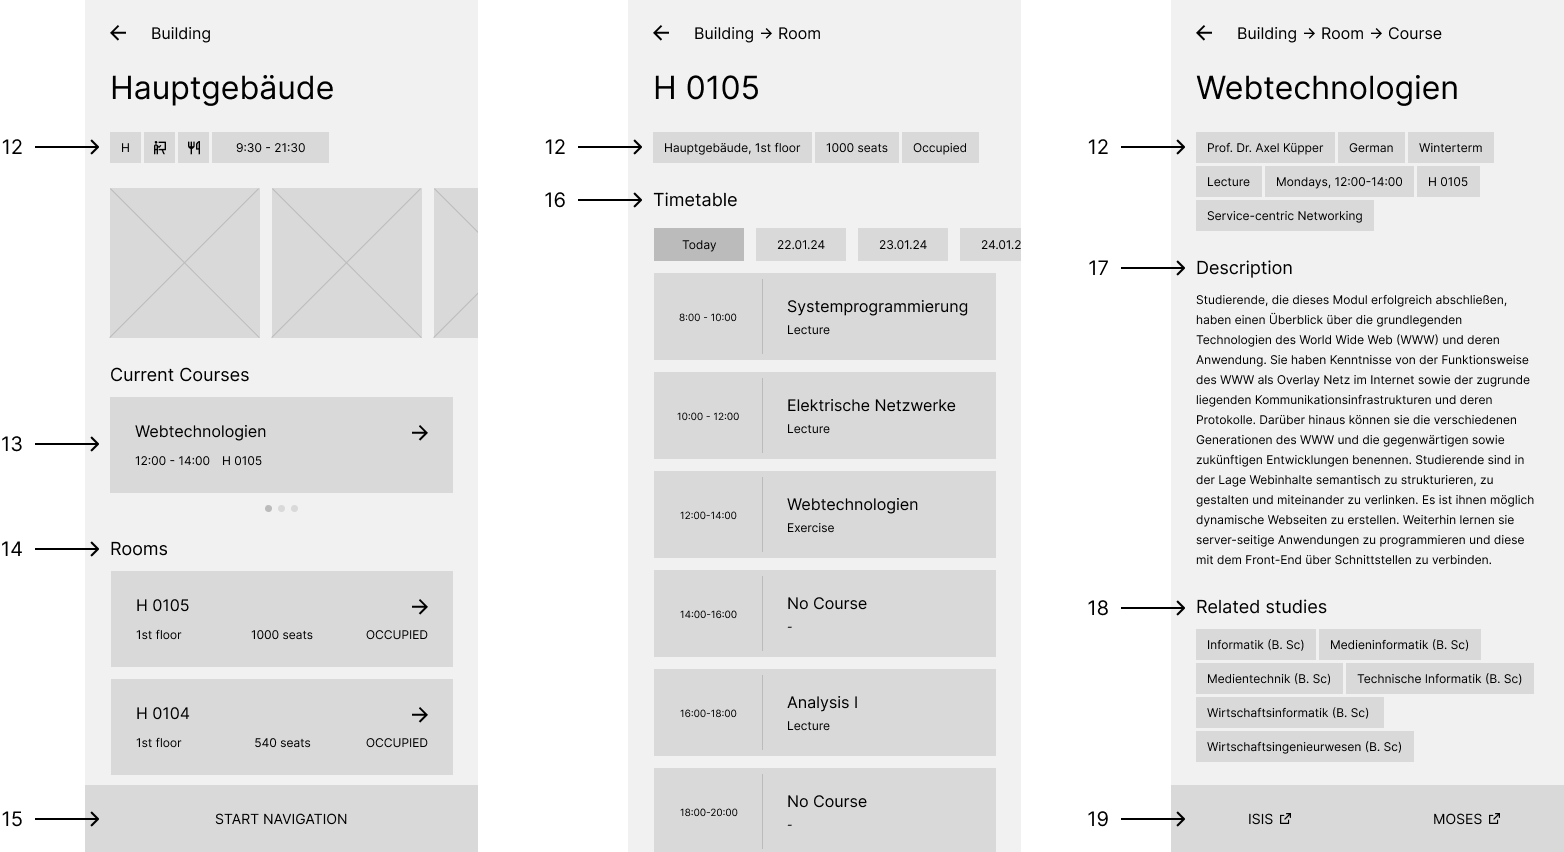
\includegraphics[width=0.9\textwidth]{images/wireframes_2.png}\\
	\caption{Most important wireframes with annotations}
\end{figure}

\begin{enumerate}
    \item Search bars are prominently placed on the main and search pages. The positioning is inspired by already established apps and enhances the UX due to \cite{jakobs_law}.
    \item To speed up the search process for certain entities, filter options are placed beneath the search bars.
    \item A button, that toggles whether the information cards are visible or not. This gives the user the decision whether to explore TU Belin's campus with the help of cards or directly by moving the map. This element also breaks down the number of choices by grouping entities by category, which, due to \cite{hicks_law}, also improves usability.
    \item Markers are placed on buildings with their respective abbreviations, the main communication symbol for buildings on TU Berlin's campus. A detailed information page is opened when clicked. They provide a sense of familiarity from other navigation services \cite{jakobs_law}.
    \item Information cards are displayed for every entity on the campus. They present the most important data of a landmark and, when in focus, move the map to the selected place and highlight it. The cards are positioned prominently on the button, to strengthen the interactivity \cite{fitts_law}.
    \item A button that toggles between 3d and 2d map perspective.
    \item A button that detects the GPS position of the user and moves the map to it.
    \item Result cards that contain different base information about the searched entities. They are sorted by category for easier search and chunking \cite{hicks_law}. A detailed information page is opened when clicked on a card.
    \item A doubled search bar, inspired by common navigation apps \cite{jakobs_law} for start and destination input.
    \item A special marker, which represents the current GPS position of the user.
    \item An overview of the calculated route, which pops up after inputting the start and the destination. It presents the most important information for the route as well as an opportunity to start the navigation. Placed on the bottom for easier access \cite{fitts_law}.
    \item Tags with the most important key facts on the detail pages for certain entities. The detail pages as well as the tags are all designed in a similar way to provide the user a structured, well-organized experience.
    \item A small pager displaying the courses, that currently take place, on the detail page for a building. They are linked to the respective course detail pages.
    \item A primary action button, prominently placed to guide the user to the navigation functionality of the app. When clicked, the app switches into navigation mode with the current building selected as the destination.
    \item A list of rooms, that can be found inside of the selected building. All cards are linked to the respective room detail pages.
    \item A timetable displaying all the courses, that take place in the selected room. It is sorted by dates. All cards are linked to the course information pages.
    \item Description and other key information on the detail page for a selected course.
    \item Further details about the course.
    \item Button options, that link to the ISIS and MOSES pages of the respective course. They are prominently placed on the bottom to allow for easy access \cite{fitts_law}.
\end{enumerate}

\section{User interface design}
The next step in the design process of the app is the user interface (UI) design. This procedure takes the already elaborated wireframes from the UX design phase and applies a consistent design language to it. One main outcome of this design step should be an identifiable corporate design of the digital product. Due to \cite{aesthetic_usability_effect}, which states that a beautifully designed user interface is perceived as a more useful one, user interface design can be seen as a subset of UX design.

Concepts to which particular attention is paid in UI design are choice of color, typography, iconography, shape-language, animation as well as usage of media, e.g., photos, videos or text. The following section and figure provide a brief specification of those parameters (often called "Styleguide") for the app design.

\begin{figure}[H]
	\centering
	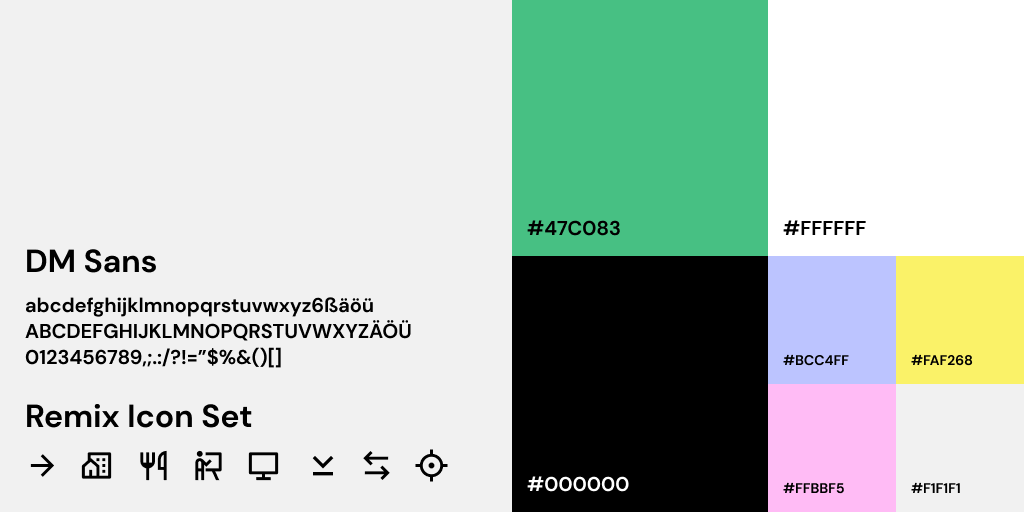
\includegraphics[width=0.85\textwidth]{images/styleguide.png}\\
	\caption{Styleguide with colors, typography and iconography}
\end{figure}

\begin{itemize}
    \item DM Sans \footnote{https://fonts.google.com/specimen/DM+Sans?query=DM+Sans} is chosen as the main font for the app, it is usually written in real black (HEX \#000000) and is used in its regular, medium and bold variations throughout the app. It occurs in font sizes 12px, 16px and 32px.
    \item The open-source Remix-Icon \footnote{https://remixicon.com} icon set with its respective Flutter package. The icons are used in their not-filled versions and set a basis for a slightly rounded design language for the entire app. Icons are consistently 20px * 20px sized and colored in HEX \#000000 black.
    \item The main color of the app is the green tone HEX \#47C083, which is supported by real black \#000000 for icons and text and real white \#FFFFFF for backgrounds and areas. Additionally, several colors representing the individual campus entities are selected: HEX \#BCC4FF (blue) for buildings, HEX \#FFBBF5 (pink) for courses, \#FAF268 (yellow) for canteens as well as HEX \#E8D4C7 (beige) for events. Furthermore, to color bigger areas inside of the white layout, two grey tones are introduced: HEX \#F1F1F1 (light grey) and HEX \#BBBBBB (dark grey) are used e.g., in a search bar, where light grey colors the element and dark grey the overlaying hint text.
    \item Animations are all 250ms long and consist of two different curves: While all map-related camera animations in Unity use a linear curve to present animation progress (camera movement over the map), the animations in the remaining user interface are based on Flutter's "Ease" curve \footnote{https://api.flutter.dev/flutter/animation/Curves/ease-constant.html}, which consists of a cubic curve mapping from [0, 1] to [0, 1] parametrized by two control points (0.25, 0.1) and (0.25, 1.0). By mimicking physical movement (which is often based on constant acceleration, e.g., gravity), the latter animation curve provides a sense of naturalness to the user while the first linear animation style makes it easier to follow the camera across the map.
    \item Usage of media: Images of TU Berlin's buildings are presented on the respective pages to provide the user with another possibility for visual reference while browsing through the app.
\end{itemize}

The following figure provides an overview of the most important screens of the final user interface design of the app.

\begin{figure}[H]
	\centering
	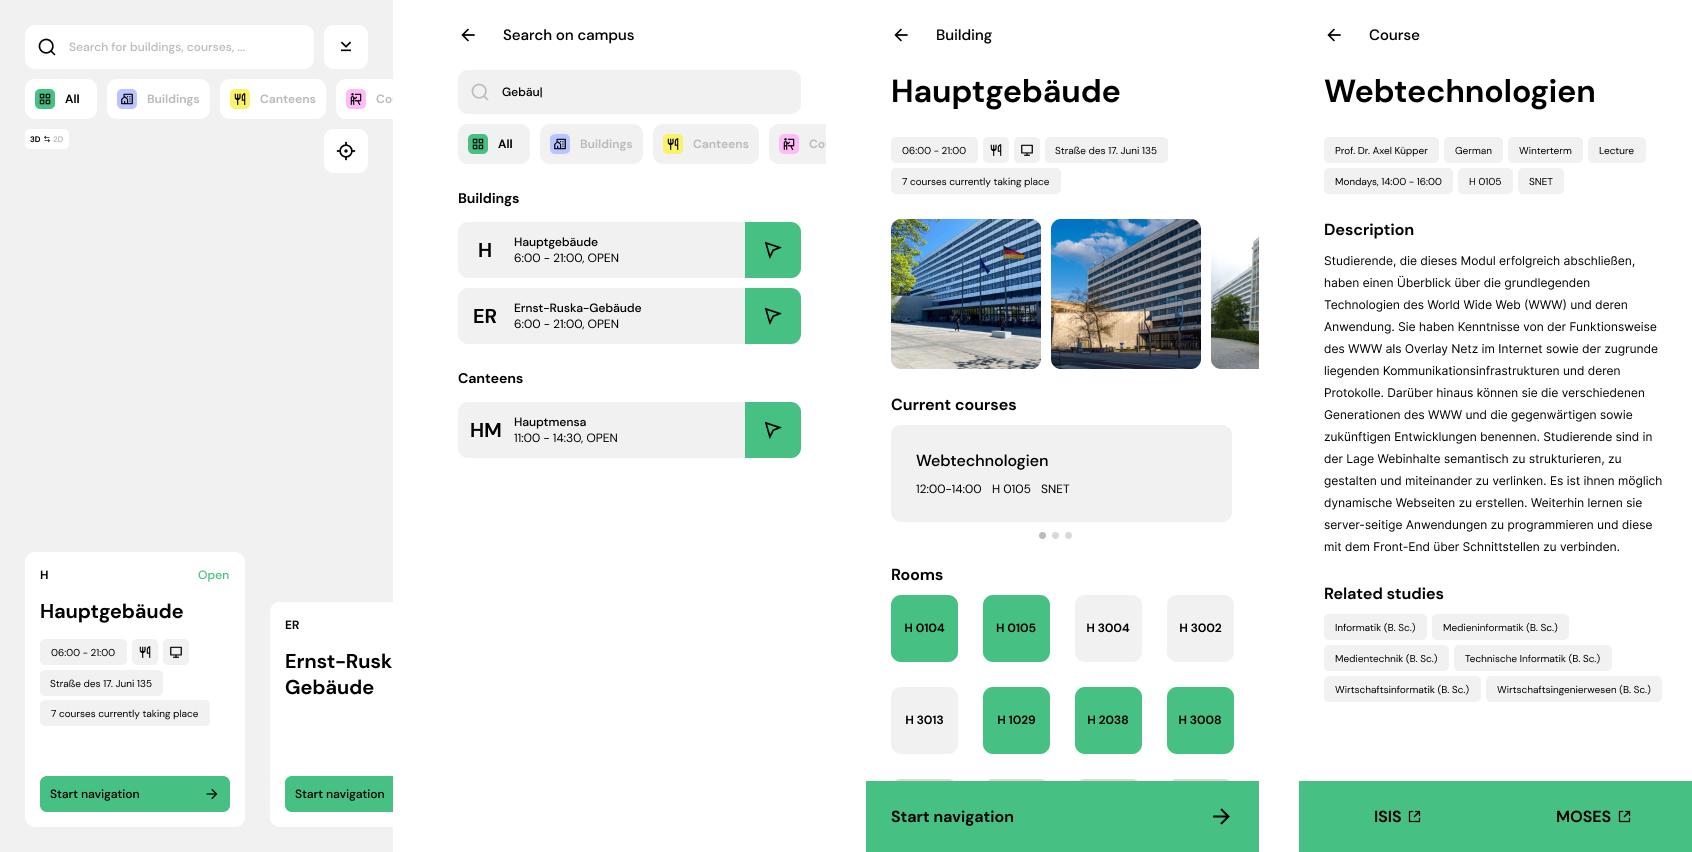
\includegraphics[width=0.85\textwidth]{images/ui_design.png}\\
	\caption{UI-Design}
\end{figure}